% !TEX root = ../main.tex
% ============================================================================
% Methodology
% ============================================================================
\chapter{Methodology}
\label{ch:method}

This chapter develops the distillation method. It first makes precise why a naive,
index-aligned distillation of HiVT's mixture output is ill-posed
(Section~\ref{ssec:method_perm}), then derives a permutation-invariant objective
(Section~\ref{ssec:method_pi}) and its two variants---the mean-target loss
(Section~\ref{ssec:method_v1}) and the distribution-matching loss
(Section~\ref{ssec:method_v2})---together with the analysis that explains why the
former breaks calibration and the latter does not. The implementation that makes
this signal reach the student reliably, and the experimental setup used to evaluate
it, are deferred to Chapter~\ref{ch:impl}.

\section{Preliminaries: HiVT's Mixture Output and Training Loss}
\label{ssec:method_prelim}
Recall from Section~\ref{ssec:sota_hivt} that, for the focal agent of a scene,
HiVT predicts a mixture of $K$ trajectory modes. Writing $\mathbf{y}\in\R^{2H}$
for a future trajectory over the $H$ prediction steps, the predicted distribution
is a Laplace mixture
\begin{equation}
  \label{eq:mixture}
  p(\mathbf{y}) \;=\; \sum_{k=1}^{K} \pi_k\,
      \Lap\!\left(\mathbf{y}\mid \loc_k, \scale_k\right),
  \qquad \pi_k \ge 0,\ \sum_{k=1}^{K}\pi_k = 1,
\end{equation}
where mode $k$ has location $\loc_k\in\R^{2H}$ (the trajectory itself), per-step
scale $\scale_k\in\R^{2H}_{>0}$ (its predicted uncertainty), and mixing
coefficient $\pi_k$. The components are the factorised, per-step Laplace densities
of Section~\ref{ssec:bg_mdn}, with $\Lap(y\mid\mu,b)=\tfrac{1}{2b}\exp(-|y-\mu|/b)$.

HiVT is trained with a regression term and a classification term. The regression
term is the Laplace negative log-likelihood (Section~\ref{ssec:bg_mle}) of the
ground-truth trajectory $\mathbf{y}^\star$ under the \emph{single best-matching}
mode---a \emph{winner-takes-all} scheme that, on each example, selects the mode
$k^\star$ closest to the ground truth and updates only its location and scale:
\begin{equation}
  \label{eq:reg}
  \mathcal{L}_{\mathrm{reg}}
    = -\frac{1}{H}\sum_{t=1}^{H}
       \log \Lap\!\left(\mathbf{y}^\star_t \mid \loc_{k^\star,t},\scale_{k^\star,t}\right),
  \qquad
  k^\star = \argmin_{k}\, \lVert \loc_k - \mathbf{y}^\star\rVert .
\end{equation}
A classification term then trains the mixing coefficients $\{\pi_k\}$ toward a
\emph{soft} target rather than a hard label on the winner: each mode is assigned a
target probability proportional to $\exp(-\bar{d}_k)$, where $\bar{d}_k$ is mode
$k$'s mean per-step displacement from the ground truth, and the predicted weights
are matched to this (stop-gradient) distribution by a cross-entropy loss.
Geometrically closer modes thus receive proportionally higher probability, with
$k^\star$ the most favoured. The per-step NLL expands to
\begin{equation}
  \label{eq:laplace_nll}
  -\log\Lap(y\mid\mu,b) = \log(2b) + \frac{|y-\mu|}{b},
\end{equation}
a form we return to in Section~\ref{ssec:method_calib}.

\section{The Mode-Permutation Problem}
\label{ssec:method_perm}
The winner-takes-all loss in~\eqref{eq:reg} supervises only one mode per example,
chosen by proximity to the ground truth. It therefore never constrains \emph{which
slot} a given behaviour occupies: across the dataset, mode index $3$ of one trained
model might capture ``turn left'' while index $3$ of another captures ``go
straight.'' The loss is, in this sense, \emph{symmetric under relabelling} of the
$K$ modes---permuting the mode indices leaves it unchanged---so two independently
trained HiVTs (such as a teacher and a student) settle on their own, mutually
unaligned slot orderings.

This is fatal for any distillation term that pairs student and teacher modes
\emph{by index}. Such a term would, for most scenes, compare a student mode against
the wrong teacher mode---``turn left'' supervised toward ``go straight''---and
inject structured noise that the model cannot resolve. Figure~\ref{fig:perm}
quantifies the misalignment on $500$ validation scenes: the per-scene optimal
matching (computed by minimum-cost linear assignment) is the identity in $0\%$ of
scenes, and pairing modes by index places them, on average, $3.98\times$ farther
apart than the optimal matching. Notably the misalignment is not random noise but a
\emph{consistent, non-identity permutation}---each student slot maps reliably to a
fixed but \emph{different} teacher slot---reflecting that both models discover a
similar repertoire of behaviours yet file them under unrelated indices. One might
imagine recovering this single global permutation once and then distilling by
index; we do not, because the correspondence is unknown a priori, drifts as the
student trains, and is not perfectly one-to-one (the unconstrained
nearest-neighbour assignment in fact falls \emph{below} chance, as several student
modes collapse onto the same teacher mode). A correct distillation objective should
instead be \emph{invariant to the ordering of both models' modes}, sidestepping any
need to estimate a correspondence at all.

\begin{figure}[htbp]
  \centering
  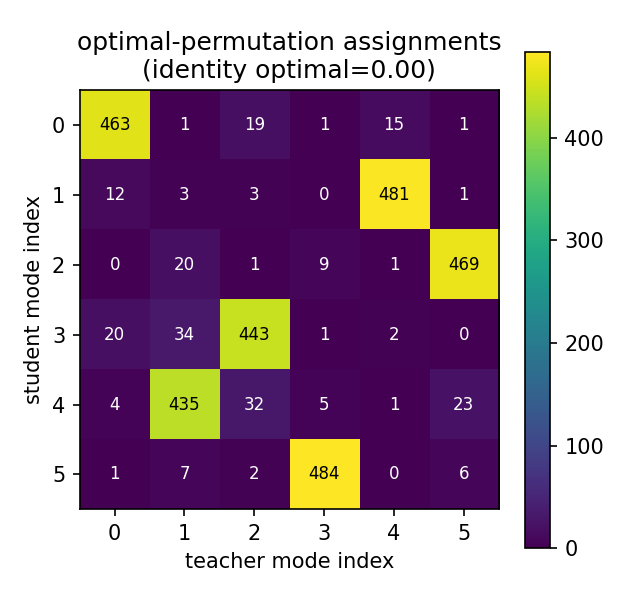
\includegraphics[width=0.6\linewidth]{figures/mode_perm_optimal.png}
  \caption{Optimal per-scene assignment between teacher (HiVT-128) and
    independently trained student (HiVT-32) mode slots, over $500$ validation
    scenes. Each cell counts how often student slot $k$ is matched to teacher slot
    $f$ under the minimum-cost one-to-one assignment (endpoint distance). The mass
    concentrates on a \emph{permuted}, non-identity diagonal: the two models learn
    a similar set of behaviours but file them under different slot indices. The
    identity permutation (slot $k\!\to\!$ slot $k$) is optimal in $0\%$ of scenes,
    and pairing modes by index is on average $3.98\times$ farther apart than the
    optimal matching ($5.16$\,m vs.\ $1.82$\,m mean endpoint distance). An
    index-aligned distillation loss would therefore mismatch modes on essentially
    every scene.}
  \label{fig:perm}
\end{figure}

\section{A Permutation-Invariant Mixture Objective}
\label{ssec:method_pi}
The resolution is to stop matching modes altogether and instead score the
teacher's predictions under the student's \emph{full mixture density}. Let the
student predict the mixture $p_S$ of~\eqref{eq:mixture} with $K_S$ modes
$\{(\pi^S_k,\loc^S_k,\scale^S_k)\}$, and let the (frozen) teacher provide $K_T$
modes $\{(\pi^T_f,\loc^T_f,\scale^T_f)\}$. The distillation objective treats the
teacher's modes as a \emph{confidence-weighted set of soft targets} and evaluates
each under $p_S$, weighting by the teacher's confidence $\pi^T_f$. This single
design choice yields the invariance we need.

\begin{prop}[Permutation invariance]
\label{prop:perm}
Any objective of the form
$\mathcal{L} = -\sum_{f=1}^{K_T} \pi^T_f\, g\!\left(p_S, \loc^T_f, \scale^T_f\right)$,
where $g$ depends on the student only through its mixture density $p_S$, is
invariant to permutations of the student's mode indices and of the teacher's mode
indices, and is well-defined when $K_S \neq K_T$.
\end{prop}
\begin{proof}
The student enters only through $p_S(\cdot)=\sum_{k}\pi^S_k\Lap(\cdot\mid\loc^S_k,\scale^S_k)$,
a sum over student modes; a finite sum is unchanged by reordering its terms, so
$p_S$---and hence $\mathcal{L}$---is invariant to permutations of the student
indices. The teacher enters only through the outer sum $\sum_f \pi^T_f(\cdot)$,
likewise invariant to reordering of the teacher indices. Neither sum refers to a
correspondence between the two index sets, so $\mathcal{L}$ requires no matching
and is defined for any $K_S,K_T$. \qed
\end{proof}

The two distillation losses below are both instances of this form; they differ
only in the choice of $g$, i.e.\ in \emph{what} of each teacher mode is scored
under $p_S$.

\section{v1: Mean-Target Distillation}
\label{ssec:method_v1}
The simplest choice scores each teacher mode's \emph{location}---the predicted
trajectory $\loc^T_f$---as a point target under the student mixture:
\begin{equation}
  \label{eq:v1}
  \mathcal{L}_{\mathrm{v1}}
    = -\sum_{f=1}^{K_T} \pi^T_f \, \log p_S\!\left(\loc^T_f\right)
    = -\sum_{f=1}^{K_T} \pi^T_f \,
        \log \sum_{k=1}^{K_S} \pi^S_k \,\Lap\!\left(\loc^T_f \mid \loc^S_k,\scale^S_k\right).
\end{equation}
This transfers \emph{where} the teacher expects the agent to go (the mode means)
and \emph{how likely} it considers each (the weights $\pi^T_f$), but it
\emph{discards the teacher's scales} $\scale^T_f$: the target is a bare point, with
no spread. By Proposition~\ref{prop:perm} it is permutation invariant. As shown
next, this objective improves best-of-$K$ geometry---the student's mode locations
are pulled toward the teacher's accurate ones---but systematically degrades
calibration.

\section{Why Mean-Target Distillation Breaks Calibration}
\label{ssec:method_calib}
The failure is a direct consequence of discarding $\scale^T_f$, and it can be read
off the Laplace NLL. Consider, for intuition, a single student mode whose location
already sits at a target $\mu$; its contribution to~\eqref{eq:v1} as a function of
its own scale $b$ is, from~\eqref{eq:laplace_nll} with $y=\mu$,
\begin{equation}
  \label{eq:shrink}
  -\log\Lap(\mu\mid\mu,b) = \log(2b),
\end{equation}
which is \emph{monotonically increasing in $b$} and minimised as $b\to 0$. Scoring a
point target thus rewards arbitrarily small scales: nothing in $\mathcal{L}_{\mathrm{v1}}$
opposes shrinkage. Contrast the baseline regression loss~\eqref{eq:laplace_nll},
where the residual term $|y-\mu|/b$ \emph{grows} as $b\to0$ whenever the prediction
is imperfect, so the two terms balance at a finite optimum.

\begin{prop}[Optimal scale of the Laplace NLL]
\label{prop:optb}
For a fixed location $\mu$ and target drawn from a distribution with
$\mathbb{E}\,|y-\mu| < \infty$, the scale minimising the expected Laplace NLL
$\mathbb{E}\!\left[\log(2b) + |y-\mu|/b\right]$ is $b^\star = \mathbb{E}\,|y-\mu|$.
\end{prop}
\begin{proof}
Differentiating $\phi(b)=\log(2b) + \mathbb{E}|y-\mu|/b$ gives
$\phi'(b)=\tfrac{1}{b}-\tfrac{\mathbb{E}|y-\mu|}{b^2}$, which vanishes at
$b=\mathbb{E}|y-\mu|$; since $\phi''(b^\star)=1/{b^\star}^2>0$ this is the unique
minimiser. \qed
\end{proof}

Proposition~\ref{prop:optb} says the well-trained baseline learns a scale that
\emph{reports its own typical error}: $b$ is a calibrated uncertainty. The
mean-target loss removes the residual term that anchors this balance, so the
student's scales are driven below their calibrated value and the predicted
intervals become too narrow---the student is \emph{over-confident}. Crucially this
is a per-mode \emph{scale} pathology, not a collapse of the mode \emph{weights}:
the argument touches only $\scale$, leaving $\{\pi_k\}$ untouched. The diagnostics
in Chapter~\ref{ch:results} confirm exactly this signature---scales shrink while
mode-weight entropy is unchanged.

\section{v2: Distribution-Matching Distillation}
\label{ssec:method_v2}
The fix is to restore the discarded spread by scoring not the bare location but
\emph{samples drawn from the teacher mode using its own scale} $\scale^T_f$. Define
\begin{equation}
  \label{eq:v2}
  \mathcal{L}_{\mathrm{v2}}
    = -\sum_{f=1}^{K_T} \pi^T_f \,
       \mathbb{E}_{\mathbf{y}\sim \Lap(\loc^T_f,\,\scale^T_f)}
        \!\left[\log p_S(\mathbf{y})\right],
\end{equation}
estimated by drawing $S$ Monte-Carlo samples per teacher mode and averaging. The
student must now place density across the \emph{whole region the teacher considers
plausible}, not merely at its centre, so collapsing its scales no longer minimises
the loss: a too-narrow student misses the teacher's outer samples and is penalised.
The objective is again of the form in Proposition~\ref{prop:perm}, hence
permutation invariant, and it relates cleanly to v1.

\begin{prop}[v2 generalises v1]
\label{prop:limit}
As the teacher scales vanish, $\scale^T_f\to\mathbf{0}$, the distribution-matching
loss~\eqref{eq:v2} reduces to the mean-target loss~\eqref{eq:v1}.
\end{prop}
\begin{proof}
As $\scale^T_f\to\mathbf{0}$ the Laplace $\Lap(\loc^T_f,\scale^T_f)$ converges to the
Dirac measure $\delta_{\loc^T_f}$, so
$\mathbb{E}_{\mathbf{y}\sim\Lap(\loc^T_f,\scale^T_f)}[\log p_S(\mathbf{y})]
\to \log p_S(\loc^T_f)$. Substituting into~\eqref{eq:v2} gives~\eqref{eq:v1}. \qed
\end{proof}

Thus v2 is the strict generalisation that v1 is the zero-variance limit of: it
transfers the teacher's full predictive distribution---locations, weights,
\emph{and} scales---and recovers v1 exactly when the teacher is certain.

\section{The Combined Objective}
\label{ssec:method_total}
In both cases the distillation term is added to HiVT's original loss with a weight
$\lambda$,
\begin{equation}
  \label{eq:total}
  \mathcal{L} = \mathcal{L}_{\mathrm{HiVT}} + \lambda\,\mathcal{L}_{\mathrm{KD}},
  \qquad \mathcal{L}_{\mathrm{KD}}\in\{\mathcal{L}_{\mathrm{v1}},\mathcal{L}_{\mathrm{v2}}\},
\end{equation}
so the student is supervised by the ground truth and the teacher simultaneously. We
note that $\lambda$ is \emph{not directly comparable across v1 and v2}: because
$\mathcal{L}_{\mathrm{v2}}$ averages a log-density over $S$ samples while
$\mathcal{L}_{\mathrm{v1}}$ scores a single point, the two terms have different
magnitudes at the same nominal $\lambda$, so an identical $\lambda$ corresponds to a
different effective distillation strength in each. The weight is therefore tuned
separately per variant (Chapter~\ref{ch:impl}).
